\section{Validation}
\begin{figure}[h]
	\centering
	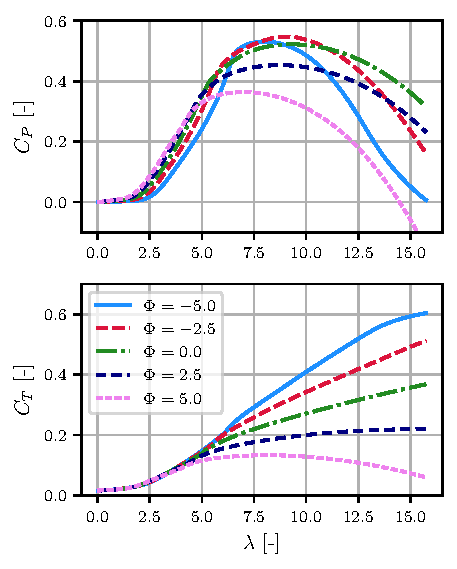
\includegraphics{cp_ct.pdf}
	\caption{$C_P$ and $C_T$ as functions of tip-speed ratio and pitch angle for the NREL 5MW turbine.}
	\label{fig:cp_+_ct}
\end{figure}
As a first step, the implementation of the BEM environment is validated. \autoref{fig:cp_+_ct} shows $C_P$ and $C_T$ computed as functions of the tip-speed ratio $\lambda$ and the collective pitch angle $\Phi$. The results appear reasonable compared to results given in \cite{hansen_aerodynamics_2008}, where a smaller turbine is used. For the NREL5 MW or any of the newer reference turbines data is not available. Furthermore, values obtained through interpolation of the precomputed table were compared to calculated values for $100$ tip-speed ratios. The difference was found to be of $\mathcal{O}\left(10^{-5}\right)$ or smaller, while the interpolation is $170$ times faster. \autoref{fig:cp_+_ct} shows that the power coefficient has a maximum between $\lambda=6$ and $\lambda=10.0$, depending on the pitch-angle. However, the thrust coefficient grows with tip-speed ratio for most pitch angles. The thrust influences the wake deficit and lifetime of wind turbines, therefore a reduction in $\lambda$ below the value maximizing $C_P$ can be advisable.\\
\begin{figure}[h]
	\centering
	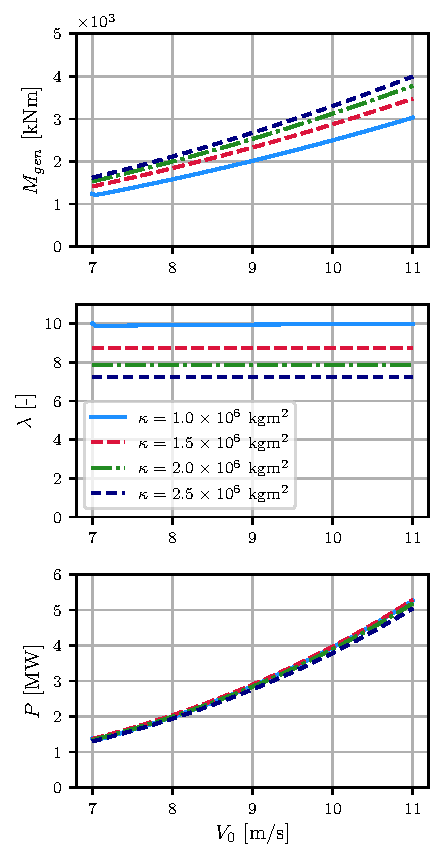
\includegraphics{greedy.pdf}
	\caption{Controller curve of greedy controller for different values of the proportionality constant $\kappa$}
	\label{fig:controller_curve}
\end{figure}
To validate the greedy controller, the controller curve is computed in the BEM environment. It is shown in \autoref{fig:controller_curve}, for a range of values of $\kappa$. The choice of $\kappa$ has little influence on the power in comparison to the wind velocity $V_0$. However, the tip-speed ratio is greatly influenced by the choice of $\kappa$. As discussed aboved, tip-speed ratio influences $C_T$ and $C_P$. Thus a higher $\kappa$ can reduce the thrust exerted on the turbine, with only a small reduction in power. Comparing the controller curve to the curve given in \cite{jonkman_definition_2009}, a good agreement in $P$ and $M_{gen}$ is found for $\kappa=\SI{2.5e6}{kgm^2}$. However, since the lifetime of the turbine is not of concern, thus $\kappa$ maximizing $C_P$,  $\kappa = \SI{1.268e6}{kgm^2}$, is chosen. \\
\begin{figure}[h]
	\centering
	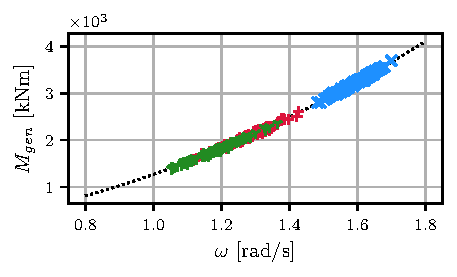
\includegraphics{control.pdf}
	\caption{Generator torque over angular velocity of three turbines controlled by greedy controller. Sampled every 200th timestep.}
	\label{fig:m_omega_greedy}
\end{figure}
The LBM-ALM with a constant angular velocity of the rotor has been validated by Asmuth et al. in \cite{asmuth_actuator_2019}. Therefore only the combination of the greedy controller with the LBM-ALM will be validated here. \autoref{fig:m_omega_greedy} shows $M_{gen}$ over $\omega$ for three turbines in a setup as described in \autoref{ssec:LBM_ALM_env}. The data gathered from the turbines agrees well with the expected value given by $\kappa \omega^2$. Deviations from the line are due to the turbulent inflow and the inertia of the turbine, but the figure shows, that the turbine can follow the changing conditions closely. Furthermore, the influence of the wake loss can be seen. While the first turbine operates near the values expected at rated wind speed, the second turbine has lower angular velocity and torque and thus generates less power. The third turbine has even lower values, although the difference between the second and third turbine is not as big as between the first and the second. \\
Thus the environments and the greedy controller exhibit the expected behaviour and the coupling of them is working as well.
